% !TEX TS-program = knitr
\documentclass[handout]{beamer}\usepackage[]{graphicx}\usepackage[]{color}
% maxwidth is the original width if it is less than linewidth
% otherwise use linewidth (to make sure the graphics do not exceed the margin)
\makeatletter
\def\maxwidth{ %
  \ifdim\Gin@nat@width>\linewidth
    \linewidth
  \else
    \Gin@nat@width
  \fi
}
\makeatother

\definecolor{fgcolor}{rgb}{0.345, 0.345, 0.345}
\newcommand{\hlnum}[1]{\textcolor[rgb]{0.686,0.059,0.569}{#1}}%
\newcommand{\hlstr}[1]{\textcolor[rgb]{0.192,0.494,0.8}{#1}}%
\newcommand{\hlcom}[1]{\textcolor[rgb]{0.678,0.584,0.686}{\textit{#1}}}%
\newcommand{\hlopt}[1]{\textcolor[rgb]{0,0,0}{#1}}%
\newcommand{\hlstd}[1]{\textcolor[rgb]{0.345,0.345,0.345}{#1}}%
\newcommand{\hlkwa}[1]{\textcolor[rgb]{0.161,0.373,0.58}{\textbf{#1}}}%
\newcommand{\hlkwb}[1]{\textcolor[rgb]{0.69,0.353,0.396}{#1}}%
\newcommand{\hlkwc}[1]{\textcolor[rgb]{0.333,0.667,0.333}{#1}}%
\newcommand{\hlkwd}[1]{\textcolor[rgb]{0.737,0.353,0.396}{\textbf{#1}}}%
\let\hlipl\hlkwb

\usepackage{framed}
\makeatletter
\newenvironment{kframe}{%
 \def\at@end@of@kframe{}%
 \ifinner\ifhmode%
  \def\at@end@of@kframe{\end{minipage}}%
  \begin{minipage}{\columnwidth}%
 \fi\fi%
 \def\FrameCommand##1{\hskip\@totalleftmargin \hskip-\fboxsep
 \colorbox{shadecolor}{##1}\hskip-\fboxsep
     % There is no \\@totalrightmargin, so:
     \hskip-\linewidth \hskip-\@totalleftmargin \hskip\columnwidth}%
 \MakeFramed {\advance\hsize-\width
   \@totalleftmargin\z@ \linewidth\hsize
   \@setminipage}}%
 {\par\unskip\endMakeFramed%
 \at@end@of@kframe}
\makeatother

\definecolor{shadecolor}{rgb}{.97, .97, .97}
\definecolor{messagecolor}{rgb}{0, 0, 0}
\definecolor{warningcolor}{rgb}{1, 0, 1}
\definecolor{errorcolor}{rgb}{1, 0, 0}
\newenvironment{knitrout}{}{} % an empty environment to be redefined in TeX

\usepackage{alltt}
\newcommand{\answers}{1}

\usetheme{Marburg}
\setbeamertemplate{navigation symbols}{} 
\setbeamertemplate{footline}
{
  \leavevmode%
  \hbox{%
  \begin{beamercolorbox}[wd=.333333\paperwidth,ht=2.25ex,dp=1ex,center]{author in head/foot}%
    \usebeamerfont{author in head/foot} $\ $ \insertshortauthor%~~\beamer@ifempty{\insertshortinstitute}{}{(\insertshortinstitute)}
  \end{beamercolorbox}%
  \begin{beamercolorbox}[wd=.333333\paperwidth,ht=2.25ex,dp=1ex,center]{title in head/foot}%
    \usebeamerfont{title in head/foot} \insertinstitute
  \end{beamercolorbox}%
  \begin{beamercolorbox}[wd=.333333\paperwidth,ht=2.25ex,dp=1ex,right]{date in head/foot}%
    \usebeamerfont{date in head/foot}\insertshortdate{}\hspace*{2em}
    \insertframenumber{} / \inserttotalframenumber\hspace*{2ex} 
  \end{beamercolorbox}}%
  \vskip0pt%
}

\usepackage{amsmath}
\usepackage{caption}
\usepackage{color}
\usepackage{enumerate}
\usepackage{listings}
\usepackage{hyperref}
\usepackage{mathrsfs}
\usepackage{natbib}
\usepackage{url}

\providecommand{\all}{\ \forall \ }
\providecommand{\bs}{\backslash}
\providecommand{\e}{\varepsilon}
\providecommand{\E}{\ \exists \ }
\providecommand{\lm}[2]{\lim_{#1 \rightarrow #2}}
\providecommand{\m}[1]{\mathbb{#1}}
\providecommand{\nv}{{}^{-1}}
\providecommand{\ov}[1]{\overline{#1}}
\providecommand{\p}{\newpage}
\providecommand{\q}{$\quad$ \newline}
\providecommand{\rt}{\rightarrow}
\providecommand{\Rt}{\Rightarrow}
\providecommand{\vc}[1]{\boldsymbol{#1}}
\providecommand{\wh}[1]{\widehat{#1}}

\hypersetup{colorlinks,linkcolor=,urlcolor=blue}
\numberwithin{equation}{section}

\definecolor{dkgreen}{rgb}{0,0.6,0}
\definecolor{gray}{rgb}{0.5,0.5,0.5}
\definecolor{mauve}{rgb}{0.58,0,0.82}

\lstset{ 
  language=C,                % the language of the code
  basicstyle= \footnotesize,           % the size of the fonts that are used for the code
  numberstyle= \tiny \color{white},  % the style that is used for the line-numbers
  stepnumber=2,                   % the step between two line-numbers. 
  numbersep=5pt,                  % how far the line-numbers are from the code
  backgroundcolor=\color{white},      % choose the background color. You must add \usepackage{color}
  showspaces=false,               % show spaces adding particular underscores
  showstringspaces=false,         % underline spaces within strings
  showtabs=false,                 % show tabs within strings adding particular underscores
  frame=lrb,                   % adds a frame around the code
  rulecolor=\color{black},        % if not set, the frame-color may be changed on line-breaks within not-black text 
  tabsize=2,                      % sets default tabsize to 2 spaces
  captionpos=t,                   % sets the caption-position 
  breaklines=true,                % sets automatic line breaking
  breakatwhitespace=false,        % sets if automatic breaks should only happen at whitespace
  %title=\lstname,                   % show the filename of files included with \lstinputlisting;
  keywordstyle=\color{blue},          % keyword style
  commentstyle=\color{gray},       % comment style
  stringstyle=\color{dkgreen},         % string literal style
  escapeinside={\%*}{*)},            % if you want to add LaTeX within your code
  morekeywords={*, ...},               % if you want to add more keywords to the set
  xleftmargin=0.053in, % left horizontal offset of caption box
  xrightmargin=-.03in % right horizontal offset of caption box
}

%\DeclareCaptionFont{white}{\color{white}}
%\DeclareCaptionFormat{listing}{\parbox{\textwidth}{\colorbox{gray}{\parbox{\textwidth}{#1#2#3}}\vskip-0.05in}}
%\captionsetup[lstlisting]{format = listing, labelfont = white, textfont = white}
%For caption-free listings, comment out the 3 lines above and uncomment the 2 lines below.
 \captionsetup{labelformat = empty, labelsep = none}
 \lstset{frame = single}




\title{More on Inference for Two-Sample Data}
\author{Yifan Zhu}
\date{}
\institute{Iowa State University}
\IfFileExists{upquote.sty}{\usepackage{upquote}}{}
\begin{document}

\begin{frame}
\titlepage
 \end{frame}
 
 \AtBeginSection[]
{
   \begin{frame}
       \frametitle{Outline}
       \tableofcontents[currentsection]
   \end{frame}
}



\section{Two-Sample Inference: Large Samples}

\begin{frame}
\frametitle{Two-sample inference}
\begin{itemize}
\item Comparing the means of two distinct populations with respect to the same measurement.
\pause \item Examples:
\begin{itemize}
\item SAT scores of high school A vs. high school B.
\pause \item Severity of a disease in women vs. in men. 
\pause \item Heights of New Zealanders vs. heights of Ethiopians.
\pause \item Coefficients of friction after wear of sandpaper A vs. sandpaper B.
\end{itemize}
\pause \item Notation:
\begin{center}
\begin{tabular}{ccc}
Sample & 1 & 2 \\ \hline
Sample size & $n_1$ & $n_2$ \\ [1ex]
True mean & $\mu_1$ & $\mu_2$ \\ [1ex] 
Sample mean & $\ov{x}_1$ & $\ov{x}_2$ \\ [1ex]
True variance & $\sigma^2_1$ & $\sigma^2_2$ \\ [1ex]
Sample variance & $s^2_1$ & $s^2_2$ 
\end{tabular}
\end{center}

\end{itemize}
\end{frame}


\begin{frame}
\frametitle{$n_1 \ge 25$ and $n_2 \ge 25$, variances known} \scriptsize
\begin{itemize}
\item We want to test $H_0: \mu_1 - \mu_2 = \#$ with some alternative hypothesis
\pause \item If $\sigma^2_1$ and $\sigma_2^2$ are known, use the test statistic:
\pause \begin{align*}
Z = \frac{(\ov{x}_1 - \ov{x}_2) - \#}{\sqrt{\frac{\sigma^2_1}{n_1} + \frac{\sigma^2_2}{n_2}}}
\end{align*}
which has a $N(0,1)$ distribution if:
\begin{itemize}
\pause \item $H_0$ is true.
\pause \item The sample 1 points are iid with mean $\mu_1$ and variance $\sigma^2_1$, the sample 2 points are iid with mean $\mu_2$ and variance $\sigma^2_2$, and the two samples are independent.
\end{itemize}
\pause \item The confidence intervals (2-sided, 1-sided upper, and 1-sided lower, respectively) for $\mu_1 - \mu_2$ are:
\begin{align*}
&\uncover<7->{\left ((\ov{x_1} - \ov{x}_2) - z_{1 - \alpha/2} \sqrt{\frac{\sigma^2_1}{n_1} + \frac{\sigma^2_2}{n_2}} , \ (\ov{x_1} - \ov{x}_2) + z_{1 - \alpha/2} \sqrt{\frac{\sigma^2_1}{n_1} + \frac{\sigma^2_2}{n_2}} \right )} \\
&\uncover<8->{\left (-\infty , \ (\ov{x_1} - \ov{x}_2) + z_{1 - \alpha} \sqrt{\frac{\sigma^2_1}{n_1} + \frac{\sigma^2_2}{n_2}} \right )} \\
&\uncover<9->{\left ((\ov{x_1} - \ov{x}_2) - z_{1 - \alpha} \sqrt{\frac{\sigma^2_1}{n_1} + \frac{\sigma^2_2}{n_2}}, \ \infty \right )} 
\end{align*}
\end{itemize}
\end{frame}


\begin{frame}
\frametitle{$n_1 \ge 25$ and $n_2 \ge 25$, variances UNknown} \scriptsize
\begin{itemize}
\item If $\sigma^2_1$ and $\sigma_2^2$ are UNknown, use the test statistic:
\pause \begin{align*}
Z = \frac{(\ov{x}_1 - \ov{x}_2) - \#}{\sqrt{\frac{s^2_1}{n_1} + \frac{s^2_2}{n_2}}}
\end{align*}
\pause \item and confidence intervals for $\mu_1 - \mu_2$:
\begin{align*}
&\uncover<4->{\left ((\ov{x_1} - \ov{x}_2) - z_{1 - \alpha/2} \sqrt{\frac{s^2_1}{n_1} + \frac{s^2_2}{n_2}} , \ (\ov{x_1} - \ov{x}_2) + z_{1 - \alpha/2} \sqrt{\frac{s^2_1}{n_1} + \frac{s^2_2}{n_2}} \right )} \\
&\uncover<5->{\left (-\infty , \ (\ov{x_1} - \ov{x}_2) + z_{1 - \alpha} \sqrt{\frac{s^2_1}{n_1} + \frac{s^2_2}{n_2}} \right )} \\
&\uncover<6->{\left ((\ov{x_1} - \ov{x}_2) - z_{1 - \alpha} \sqrt{\frac{s^2_1}{n_1} + \frac{s^2_2}{n_2}}, \ \infty \right )} 
\end{align*}
\end{itemize}
\end{frame}



\section{Two-Sample Inference: Small samples}

\begin{frame}
\frametitle{Small samples and $\sigma^2_1 = \sigma^2_2 = \sigma^2$ (UNknown)}
\begin{itemize}
\item Assuming $\sigma^2_1 = \sigma^2_2 = \sigma^2$, then we can use the {\bf pooled sample variance} to estimate $\sigma^2$,
\pause \begin{align*}
s^2_p = \frac{(n_1 - 1) s_1^2 + (n_2 - 1) s_2^2}{n_1 + n_2 - 2}
\end{align*}
\pause \item A test statistic to test $H_0: \mu_1 - \mu_2 = \#$ against some alternative is:
\pause \begin{align*}
T = \frac{\ov{x}_1 - \ov{x}_2 - \#}{s_p \sqrt{\frac{1}{n_1} + \frac{1}{n_2}}}
\end{align*}
\pause \item $T \sim t_{n_1 + n_2 -2}$ assuming:
\begin{itemize}
\pause \item $H_0$ is true.
\pause \item The sample 1 points are iid $N(\mu_1, \sigma^2)$, the sample 2 points are iid $N(\mu_2, \sigma^2$), and the sample 1 points are independent of the sample 2 points.
\end{itemize}
\end{itemize}
\end{frame}

\begin{frame}
\frametitle{Small samples and $\sigma^2_1 = \sigma^2_2 = \sigma^2$ (UNknown)} \scriptsize
\begin{itemize}
\item $1 - \alpha$ confidence intervals (2-sided, 1-sided upper, and 1-sided lower, respectively) for $\mu_1 - \mu_2$ under these assumptions are of the form: 
\end{itemize}
\begin{align*}
&\uncover<2->{\left ((\ov{x_1} - \ov{x}_2) - t_{\nu, \ 1 - \alpha/2} s_p \sqrt{\frac{1}{n_1} + \frac{1}{n_2}} , \ (\ov{x_1} - \ov{x}_2) + t_{\nu, \ 1 - \alpha/2} s_p \sqrt{\frac{1}{n_1} + \frac{1}{n_2}} \right )} \\
&\uncover<3->{\left (-\infty , \ (\ov{x_1} - \ov{x}_2) + t_{\nu, \ 1 - \alpha} s_p \sqrt{\frac{1}{n_1} + \frac{1}{n_2}} \right )} \\
&\uncover<4->{\left ((\ov{x_1} - \ov{x}_2) - t_{\nu, \ 1 - \alpha} s_p \sqrt{\frac{1}{n_1} + \frac{1}{n_2}}, \ \infty \right )}
\end{align*}
\uncover<4->{where $\nu = n_1 + n_2 - 2$.}
\end{frame}






\begin{frame}
\frametitle{Example: springs}
\begin{itemize}
\item The data of W. Armstrong on spring lifetimes (appearing in the book by Cox and Oakes) not only concern spring longevity at a 950 N/mm2 stress level but also longevity at a 900 N/mm2 stress level. 
\end{itemize}
\begin{center}
\setkeys{Gin}{width=.8\textwidth} 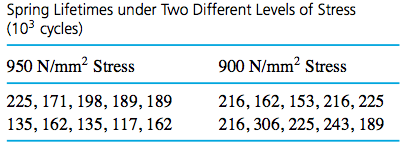
\includegraphics{../../fig/springdata.png}
\end{center}
\begin{itemize}
\pause \item Let sample 1 be the 900 N/mm${}^2$ stress group and sample 2 be the 950 N/mm${}^2$ stress group.
\pause \item $\ov{x}_1 = 215.1, \ov{x}_2 = 168.3$.
\pause \item Let's do a hypothesis test to see if the sample 1 springs lasted significantly longer than the sample 2 springs.
\end{itemize}
\end{frame}

\begin{frame}
\frametitle{\small Check normality and homogeneity of variances}
\scriptsize
Make a normal Q-Q plot of both sample on the same plot. If both sample look like a straight line and these two lines are almost parallel, then it is plausible that both sample are normally distributed with equal variancec.
\setkeys{Gin}{width=.8\textwidth} 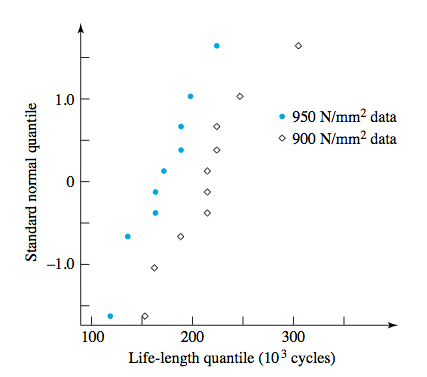
\includegraphics{../../fig/springsqq.png}
\end{frame}
















\begin{frame}
\frametitle{Example: springs}
\begin{enumerate}[1. ]
\item $H_0:  \mu_1 - \mu_2 = 0$, $H_a: \mu_1 - \mu_2 > 0$.
\pause \item $\alpha = 0.05$
\pause \item The test statistic is:
\pause \begin{align*}
T = \frac{(\ov{x}_1 - \ov{x}_2) - 0}{s_p \sqrt{\frac{1}{n_1} + \frac{1}{n_2}}}
\end{align*}
\begin{itemize}
\pause \item Assume:
\begin{itemize}
\pause \item $H_0$ is true.
\pause \item The sample 1 spring lifetimes are iid $N(\mu_1, \sigma^2)$
\pause \item The sample 2 spring lifetimes are iid $N(\mu_2, \sigma^2)$
\pause \item The sample 1 spring lifetimes are independent of those of sample 2.
\end{itemize}
\pause \item Under these assumptions, $T \sim t_{n_1 + n_2 - 2} = t_{10 + 10 - 2} = t_{18}$.
\pause \item Reject $H_0$ if $T > t_{18, \ 1 - \alpha}$
\end{itemize}
\newcounter{saveenum}
\setcounter{saveenum}{\value{enumi}}

\end{enumerate}
\end{frame}

\begin{frame}
\frametitle{Example: springs} \scriptsize
\begin{align*}
s_1 &= \sqrt{\frac{1}{n_1 - 1} \sum_i (x_{1, i} - \ov{x}_1)^2} \\
&\uncover<2->{ \qquad = \sqrt{\frac{1}{9} (225 - 215.1)^2 + (171 - 215.1)^2 + \cdots + (162 - 215.1)^2}}\uncover<3->{ = 42.9 }\\
\uncover<4->{s_2} & \uncover<4->{= \sqrt{\frac{1}{n_2 - 1} \sum_i (x_{2, i} - \ov{x}_2)^2}}\\
& \uncover<5->{\qquad = \sqrt{\frac{1}{9} (225 - 168.3)^2 + (171 - 168.3)^2 + \cdots + (162 - 168.3)^2}} \uncover<6->{= 33.1}\\
\uncover<7->{s_p} &\uncover<7->{= \sqrt{ \frac{(10-1)42.9^2+ (10-1)33.1^2}{10 + 10 - 2}}} \uncover<8->{= 38.3}
\end{align*}
\end{frame}


\begin{frame}
\frametitle{Example: springs}
\begin{enumerate}[1. ]
 \setcounter{enumi}{\value{saveenum}}
\item 
\begin{align*}
\uncover<2->{t} & \uncover<2->{=  \frac{(\ov{x}_1 - \ov{x}_2) - 0}{s_p \sqrt{\frac{1}{n_1} + \frac{1}{n_2}}}} \uncover<3->{ = \frac{215.1 - 168.3 - 0}{38.3 \cdot \sqrt{\frac{1}{10} + \frac{1}{10}}}} \uncover<4->{= 2.7} \\
\uncover<5->{t_{18, \ 1 - \alpha}} & \uncover<6->{= t_{18, \ 1 - 0.05}}  \uncover<7->{= t_{18, \ 0.95}}  \\
&\uncover<8->{= 1.73}
\end{align*}
\uncover<9->{\item With $t = 2.7 > 1.73 = t_{18, 0.95}$, we reject $H_0$ in favor of $H_a$.}
\uncover<10->{\item There is enough evidence to conclude that springs last longer if subjected to 900 $N/mm^2$ of stress than if subjected to 950 $N/mm^2$ of stress.}
\end{enumerate}
\end{frame}


\begin{frame}
\frametitle{Example: springs} \scriptsize
\begin{itemize}
\item A 95\%, 2-sided confidence interval for the difference in lifetimes is:
\end{itemize}
\begin{align*}
&\uncover<2->{\left ((\ov{x_1} - \ov{x}_2) - t_{\nu, \ 1 - \alpha/2} s_p \sqrt{\frac{1}{n_1} + \frac{1}{n_2}} , \ (\ov{x_1} - \ov{x}_2) + t_{\nu, \ 1 - \alpha/2} s_p \sqrt{\frac{1}{n_1} + \frac{1}{n_2}} \right )} \\
\intertext{\uncover<3->{Using $t_{\nu, \ 1 - \alpha/2} = t_{18, 1 - 0.05/2} = t_{18, \ 0.975} = 2.1$:}}
&\uncover<4->{\left ((215.1 - 168.3) - 2.1 \cdot 38.3 \sqrt{\frac{1}{10} + \frac{1}{10}} , (215.1 - 168.3) + 2.1 \cdot 38.3 \sqrt{\frac{1}{10} + \frac{1}{10}} \right )} \\
&\uncover<5->{=  (10.8, 82.8)}
\end{align*}
\begin{itemize}
\uncover<6->{\item We are $95\%$ confident that the springs subjected to 900 $N/mm^2$ of stress last between $10.8 \times 10^3$ and $82.8 \times 10^3$ cycles longer than the springs subjected to 950 $N/mm^2$ of stress.}
\end{itemize}
\end{frame}
















\begin{frame}
\frametitle{Your turn: stopping distances}
\begin{itemize}
\item Suppose $\mu_1$ and $\mu_2$ are true mean stopping distances (in meters) at 50 mph for cars of a certain type equipped with two different types of breaking systems. 
\pause \item Suppose $n_1 = n_2 = 6, \ov{x}_1 = 115.7, \ov{x}_2 = 129.3, s_1 = 5.08, s_2 = 5.38$.
\pause \item Use significance level 0.01 to test $H_0: \mu_1 - \mu_2 = -10$ vs. $H_a: \mu_1 - \mu_2 < -10$. 
\pause \item Construct a 2-sided 99\% confidence interval for the true difference in stopping distances.
\end{itemize}
\end{frame}





\begin{frame}<handout:\answers>
\frametitle{Answers: stopping distances}
\begin{enumerate}[1. ]
\item $H_0:  \mu_1 - \mu_2 = -10$, $H_a: \mu_1 - \mu_2 < -10$. 
\pause \item $\alpha = 0.01$
\pause \item The test statistic is:
\pause \begin{align*}
T = \frac{(\ov{x}_1 - \ov{x}_2) - (-10)}{s_p \sqrt{\frac{1}{n_1} + \frac{1}{n_2}}}
\end{align*}
\begin{itemize}
\pause \item Assume:
\begin{itemize}
\pause \item $H_0$ is true.
\pause \item The sample 1 stopping distances are iid $N(\mu_1, \sigma^2)$
\pause \item The sample 2 stopping distances are iid $N(\mu_2, \sigma^2)$
\pause \item The sample 1 stopping distances are independent of those of sample 2.
\end{itemize}
\pause \item Under these assumptions, $T \sim t_{n_1 + n_2 - 2} = t_{6 + 6 - 2} = t_{10}$.
\pause \item Reject $H_0$ if $T < t_{10, \  \alpha}$
\end{itemize}
\setcounter{saveenum}{\value{enumi}}
\end{enumerate}
\end{frame}


\begin{frame}<handout:\answers>
\frametitle{Answers: stopping distances}
\begin{itemize}
\item $s_1 = 5.08$, $s_2 = 5.38$.
\item 
\begin{align*}
\uncover<2->{s_p} &\uncover<2->{= \sqrt{\frac{(n_1 - 1)s_1^2 + (n_2 - 1)s_2^2}{n_1 + n_2 - 2}}} \\
 &\uncover<3->{ \qquad = \sqrt{\frac{(6 - 1)(5.08)^2 + (6 - 1)(5.38)^2}{6 + 6 - 2}} }\\
 &\uncover<4->{ \qquad = 5.23}
\end{align*}
\end{itemize}
\end{frame}



\begin{frame}<handout:\answers>
\frametitle{Answers: stopping distances} \small
\begin{enumerate}[1. ]
 \setcounter{enumi}{\value{saveenum}}
\item
\begin{align*}
\uncover<2->{t} & \uncover<2->{=  \frac{(\ov{x}_1 - \ov{x}_2) - (-10)}{s_p \sqrt{\frac{1}{n_1} + \frac{1}{n_2}}}}\uncover<3->{ = \frac{115.7 - 129.3 +10 }{5.23 \cdot \sqrt{\frac{1}{6} + \frac{1}{6}}}} \uncover<4->{ = -1.19 }\\
\uncover<5->{t_{10, \ 1 - \alpha}} & \uncover<6->{= t_{10, \ 0.99}} \uncover<7->{ = -2.76}  \\
\end{align*}
\uncover<8->{\item With $t = -1.19 \not  < -2.76 = t_{10, 0.99}$, we reject $H_0$ in favor of $H_a$.}
\uncover<9->{\item There is not enough evidence to conclude that the stopping distances of breaking system 1 are less than those of breaking system 2 by over 10 meters.  }
\end{enumerate}
\end{frame}


\begin{frame}<handout:\answers>
\frametitle{Answers: stopping distances} \scriptsize
\begin{itemize}
\item A 99\%, 2-sided confidence interval for the difference in breaking distances is:
\end{itemize}
\begin{align*}
&\uncover<2->{\left ((\ov{x_1} - \ov{x}_2) - t_{\nu, \ 1 - \alpha/2} s_p \sqrt{\frac{1}{n_1} + \frac{1}{n_2}} , \ (\ov{x_1} - \ov{x}_2) + t_{\nu, \ 1 - \alpha/2} s_p \sqrt{\frac{1}{n_1} + \frac{1}{n_2}} \right )} \\
\intertext{\uncover<3->{Using $t_{\nu, \ 1 - \alpha/2} = t_{10, 1 - 0.01/2} = t_{10, \ 0.995} = 3.17$:}}
&\uncover<4->{\left ((115.7 - 129.3) - 3.17 \cdot 5.23 \sqrt{\frac{1}{6} + \frac{1}{6}} , (115.7 - 129.3) + 3.17 \cdot 5.23 \sqrt{\frac{1}{6} + \frac{1}{6}} \right )} \\
&\uncover<5->{=  (-23.17, -4.03)}
\end{align*}
\begin{itemize}
\uncover<6->{\item We are $99\%$ confident that the true mean stopping distance of breaking system 1 is anywhere from 23.17 m to 4.03 m less than that of breaking system 2.}
\end{itemize}
\end{frame}































%%%% cochran-satterthwaite




\begin{frame}
\frametitle{What if $\sigma_1^2 \ne \sigma_2^2$?} \small
\begin{itemize}

\pause \item The test statistic for testing $H_0: \mu_1 - \mu_2 = \#$ vs. some $H_a$ is:
\pause \begin{align*}
T = \frac{\ov{x}_1 - \ov{x}_2 - \#}{\sqrt{\frac{s_2^2}{n_2} + \frac{s_1^2}{n_1}}}
\end{align*}
Under the assumptions that:
\begin{itemize}
\pause \item $H_0$ is true.
\pause \item The sample 1 observations are iid $N(\mu_1, \sigma^2_1)$ and the sample 2 observations are iid $N(\mu_2, \sigma^2_2)$
\end{itemize}
The test statistic has an approximate $t_{\hat{\nu}}$ distribution, where the degrees of freedom is estimated
by the following special case of the Cochran-Satterthwaite
approximation for linear combinations of mean squares:
\[\hat{\nu} = \frac{\left(\frac{s_1^2}{n_1} + \frac{s_2^2}{n_2}\right)^2}{\frac{s_1^4}{(n_1 - 1)n_1^2} + \frac{s_2^4}{(n_2 - 1)n_2^2}}\]

\end{itemize}
\end{frame}


\begin{frame}
\frametitle{What if $\sigma_1^2 \ne \sigma_2^2$?} \scriptsize
\begin{itemize}
\item Under these assumptions, the $1 - \alpha$ confidence intervals for $\mu_1 - \mu_2$ become:
\end{itemize}
\begin{align*}
&\uncover<2->{\left ((\ov{x_1} - \ov{x}_2) - t_{\wh{\nu}, \ 1 - \alpha/2}  \sqrt{\frac{s_1^2}{n_1} + \frac{s_2^2}{n_2}} , \ (\ov{x_1} - \ov{x}_2) + t_{\wh{\nu}, \ 1 - \alpha/2} \sqrt{\frac{s_1^2}{n_1} + \frac{s_2^2}{n_2}} \right )} \\
&\uncover<3->{\left (-\infty , \ (\ov{x_1} - \ov{x}_2) + t_{\wh{\nu}, \ 1 - \alpha} \sqrt{\frac{s_1^2}{n_1} + \frac{s_2^2}{n_2}} \right )} \\
&\uncover<4->{\left ((\ov{x_1} - \ov{x}_2) - t_{\wh{\nu}, \ 1 - \alpha} \sqrt{\frac{s_1^2}{n_1} + \frac{s_2^2}{n_2}}, \ \infty \right ) }
\end{align*}
\end{frame}









\begin{frame}
\frametitle{Example: springs}
\begin{itemize}
\item In the springs example, $\sigma_1^2$ probably doesn't equal $\sigma_2^2$ because $s_1 = 57.9$ and $s_2 = 33.1$.
\pause \item I'll redo the hypothesis test and the confidence interval using: 
\begin{align*}
\uncover<3->{\wh{\nu}} \uncover<3->{= \frac{\left (\frac{s_1^2}{n_1} + \frac{s_2^2}{n_2} \right )^2}{\frac{s_1^4}{(n_1 - 1)n_1^2} + \frac{s_2^4}{(n_2 - 1)n_2^2}}} \uncover<4->{ = \frac{\left (\frac{57.9^2}{10} + \frac{33.1^2}{10} \right )^2}{\frac{57.9^4}{(10 - 1)10^2} + \frac{33.1^4}{(10 - 1)10^2}}} \uncover<5->{ =14.3}
\end{align*}
\end{itemize}
\end{frame}



\begin{frame}
\frametitle{Example: springs}
\begin{enumerate}[1. ]
\item $H_0:  \mu_1 - \mu_2 = 0$, $H_a: \mu_1 - \mu_2 > 0$.
\pause \item $\alpha = 0.05$
\pause \item The test statistic is:
\pause \begin{align*}
T = \frac{(\ov{x}_1 - \ov{x}_2) - 0}{ \sqrt{\frac{s_1^2}{n_1} + \frac{s_2^2}{n_2}}} 
\end{align*}
\begin{itemize}
\pause \item Assume:
\begin{itemize}
\pause \item $H_0$ is true.
\pause \item The sample 1 spring lifetimes are $N(\mu_1, \sigma^2_1)$
\pause \item The sample 2 spring lifetimes are $N(\mu_2, \sigma^2_2)$
\pause \item The sample 1 spring lifetimes are independent of those of sample 2.
\end{itemize}
\pause \item Under these assumptions, $T \sim t_{\wh{\nu}} = t_{14.3}$.
\pause \item Reject $H_0$ if $T > t_{14.3, \ 1 - \alpha}$
\end{itemize}
\setcounter{saveenum}{\value{enumi}}

\end{enumerate}
\end{frame}

\begin{frame}
\frametitle{Example: springs}
\begin{enumerate}[1. ]
 \setcounter{enumi}{\value{saveenum}}
\item The moment of truth:
\begin{align*}
\uncover<2->{t} & \uncover<2->{=  \frac{(\ov{x}_1 - \ov{x}_2) - 0}{ \sqrt{\frac{s_1^2}{n_1} + \frac{s_2^2}{n_2}}}} \uncover<3->{ = \frac{215.1 - 168.3 - 0}{ \sqrt{\frac{57.9^2}{10} + \frac{33.1^2}{10}}}} \uncover<4->{ = 2.22} \\
\uncover<5->{t_{14.3, \ 1 - \alpha}} & \uncover<6->{= t_{14.3, \ 1 - 0.05}} \uncover<7->{ = t_{14.3, \ 0.95}}  \\
&\uncover<8->{= 1.76 \quad \text{\scriptsize (Take $\nu = 14$ if you're using the t table)}}
\end{align*}
\uncover<9->{\item With $t = 2.22 > 1.76 = t_{14.3, 0.95}$, we reject $H_0$ in favor of $H_a$.}
\uncover<10->{\item There is still enough evidence to conclude that springs last longer if subjected to 900 $N/mm^2$ of stress than if subjected to 950 $N/mm^2$ of stress.}
\end{enumerate}
\end{frame}


\begin{frame}
\frametitle{Example: springs} \scriptsize
\begin{itemize}
\item A 95\%, 2-sided confidence interval for the difference in lifetimes is:
\end{itemize}
\begin{align*}
&\uncover<2->{\left ((\ov{x_1} - \ov{x}_2) - t_{\wh{\nu}, \ 1 - \alpha/2} \sqrt{\frac{s_1^2}{n_1} + \frac{s_2^2}{n_2}} , \ (\ov{x_1} - \ov{x}_2) + t_{\wh{\nu}, \ 1 - \alpha/2} \sqrt{\frac{1}{n_1} + \frac{1}{n_2}} \right )} \\
\intertext{\uncover<3->{Using $t_{\wh{\nu}, \ 1 - \alpha/2} = t_{14.3, \ 1 - 0.05/2} = t_{14.3, 0.975} = 2.14$:}}
&\uncover<4->{\left ((215.1 - 168.3) - 2.14 \cdot  \sqrt{\frac{57.9^2}{10} + \frac{33.1^2}{10}} , \right .} \\ 
&\uncover<5->{ \qquad \left . (215.1 - 168.3) + 2.14 \cdot  \sqrt{\frac{57.9^2}{10} + \frac{33.1^2}{10}} \right )} \\
&\uncover<6->{=  (1.67, \ 91.9)}
\end{align*}
\begin{itemize}
\uncover<7->{\item We are $95\%$ confident that the springs subjected to 900 $N/mm^2$ of stress last between $1.67 \times 10^3$ and $91.1 \times 10^3$ cycles longer than the springs subjected to 950 $N/mm^2$ of stress.}
\end{itemize}
\end{frame}




\begin{frame}
\frametitle{Your turn: fabrics} \scriptsize
\begin{itemize}
\item The void volume within a textile fabric affects comfort, flammability, and insulation properties. Permeability ($cm^3/cm^2/s$) of a fabric refers to the accessibility of void space to the flow of a gas or liquid. 
\pause \item Consider the following data on two different types of plain-weave fabric:
\end{itemize}
\setkeys{Gin}{width=1\textwidth} 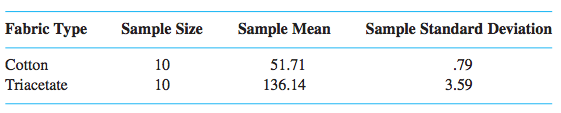
\includegraphics{../../fig/fabricdata.png}
\begin{itemize}
\pause \item Let Sample 1 be the triacetate fabric and Sample 2 be the cotton fabric.
\pause \item Using $\alpha = 0.05$, attempt to verify the claim that triacetate fabrics are more permeable than the cotton fabrics on average.
\pause \item Construct and interpret a two-sided 95\% confidence interval for the true difference in mean permeability.
\end{itemize}
\end{frame}



\begin{frame}<handout:\answers>
\frametitle{Answers: fabrics}
\begin{itemize}
\item $n_1 = n_2 = 10$.
\pause \item $\ov{x}_1 = 136.14$, $\ov{x}_2 = 51.71$.
\pause \item $s_1 = 3.59$, $s_2 = 0.79$.
\item
\begin{align*}
\uncover<4->{\wh{\nu} = \frac{\left (\frac{s_1^2}{n_1} + \frac{s_2^2}{n_2} \right )^2}{\frac{s_1^4}{(n_1 - 1)n_1^2} + \frac{s_2^4}{(n_2 - 1)n_2^2}}} \uncover<5->{ = \frac{\left (\frac{3.59^2}{10} + \frac{0.79^2}{10} \right )^2}{\frac{3.59^4}{(10 - 1)10^2} + \frac{0.79^4}{(10 - 1)10^2}}} \uncover<6->{ = 9.87}
\end{align*}
\uncover<7->{\item If you're using the t table, round down to $\nu = 9$ to avoid unneccessary false positives.}
\end{itemize}
\end{frame}















\begin{frame}<handout:\answers>
\frametitle{Answers fabrics}
\begin{enumerate}[1. ]
\item $H_0:  \mu_1 - \mu_2 = 0$, $H_a: \mu_1 - \mu_2 > 0$.
\pause \item $\alpha = 0.05$
\pause \item The test statistic is:
\pause \begin{align*}
T = \frac{(\ov{x}_1 - \ov{x}_2) - 0}{ \sqrt{\frac{s_1^2}{n_1} + \frac{s_2^2}{n_2}}} 
\end{align*}
\begin{itemize}
\pause \item Assume:
\begin{itemize}
\pause \item $H_0$ is true.
\pause \item The triacetate permeabilities are $N(\mu_1, \sigma^2_1)$
\pause \item The cotton permeabilities are $N(\mu_2, \sigma^2_2)$
\pause \item The triacetate permeabilities are independent of the cotton permeabilities.
\end{itemize}
\pause \item Under these assumptions, $T \sim t_{\wh{\nu}} = t_{9.87}$.
\pause \item Reject $H_0$ if $T > t_{9.87, \ 1 - \alpha}$
\end{itemize}
\setcounter{saveenum}{\value{enumi}}

\end{enumerate}
\end{frame}

\begin{frame}<handout:\answers>
\frametitle{Answers fabrics}
\begin{enumerate}[1. ]
\setcounter{enumi}{\value{saveenum}}
\item 
\begin{align*}
\uncover<2->{t} & \uncover<2->{=  \frac{(\ov{x}_1 - \ov{x}_2) - 0}{ \sqrt{\frac{s_1^2}{n_1} + \frac{s_2^2}{n_2}}}} \uncover<3->{= \frac{136.14 - 51.71 - 0}{ \sqrt{\frac{3.59^2}{10} + \frac{0.79^2}{10}}}} \uncover<4->{ = 72.63} \\
&\uncover<5->{t_{9.87, \ 1 - \alpha} \approx  t_{9, 1- \alpha}} \uncover<6->{ = t_{9, \ 0.95}} \uncover<7->{ =  1.83} \\
\end{align*}
\uncover<8->{\item With $t = 72.63 > 1.83 = t_{9, 0.95}$, we reject $H_0$ in favor of $H_a$.}
\uncover<9->{\item There is overwhelming evidence to conclude that the triacetate fabrics are more permeable than the cotton fabrics.}
\end{enumerate}
\end{frame}


\begin{frame}<handout:\answers>
\frametitle{Answers fabrics} \scriptsize
\begin{itemize}
\item With $t_{\wh{\nu}, 1 - \alpha/2} \approx t_{9, 0.975 }= 2.26$, a 95\%, 2-sided confidence interval for the difference in lifetimes is:
\end{itemize}
\begin{align*}
&\uncover<2->{\left ((\ov{x_1} - \ov{x}_2) - t_{\wh{\nu}, \ 1 - \alpha/2} \sqrt{\frac{s_1^2}{n_1} + \frac{s_2^2}{n_2}} , \ (\ov{x_1} - \ov{x}_2) + t_{\wh{\nu}, \ 1 - \alpha/2} \sqrt{\frac{s^2_1}{n_1} + \frac{s^2_2}{n_2}} \right )} \\
&\uncover<3->{\left ((136.14 - 51.71) - 2.26 \cdot  \sqrt{\frac{3.59^2}{10} + \frac{0.79^2}{10}} , \right .} \\ 
& \uncover<4->{\qquad \left . (136.14 - 51.71) + 2.26 \cdot  \sqrt{\frac{3.59^2}{10} + \frac{0.79^2}{10}} \right )} \\
&\uncover<5->{=  (81.80, \ 87.06) }
\end{align*}
\begin{itemize}
\uncover<6->{\item We are $95\%$ confident that the permeability of the triacetate fabric exceeds that of the cotton fabric by anywhere between 81.80 $cm^3/cm^2/s$ and 87.06 $cm^3/cm^3/s$.}
\end{itemize}
\end{frame}










\end{document}
